% https://www.urionlinejudge.com.br/judge/en/problems/view/1168
\NomeProblema{LED Fácil}%

Um \emph{diodo emissor de luz} (LED) pode ser usado como uma lâmpada extremamente 
eficiente em um letreiro, e D'Barros quer montar um painel mostrando a quantidade 
de clientes que ele atendeu em sua lojinha antes de se aposentar. Ele não possui 
muitos LEDs, e não tem certeza se conseguirá montar o número desejado. Considerando 
a configuração de LEDs dos números abaixo (cada traço é um LED), faça um algoritmo 
que ajude D'Barros a descobrir o número de LEDs necessário para exibir tal valor.

\begin{center}
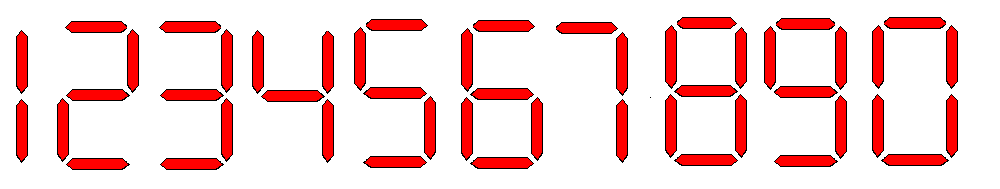
\includegraphics[width=.8\textwidth]{leds}%
\end{center}%

\subsection*{Entrada}%
A entrada contém um inteiro $N$, $(1 <= N <= 2\cdot10^6)$, correspondendo a quantidade de
clientes atendidos por D'Barros.

\subsection*{Saída}%
Mostre uma linha contendo o número de LEDs que D'Barros precisará para exibir a
quantidade desejada, seguido pela palavra ``LEDs'' (e quebra de linha!).

% \setInputWidth{.1\textwidth}%